%
% $Id: $
%
%
% Compilar a .pdf con LaTeX (pdflatex)
% Es necesario instalar Beamer (paquete latex-beamer en Debian)
%

%
% Gráficos:
% Los gráficos pueden suministrarse en PNG, JPG, TIF, PDF, MPS
% Los EPS deben convertirse a PDF (usar epstopdf)
%

\documentclass{beamer}
\usetheme{Warsaw}
\usebackgroundtemplate{
\includegraphics[width=\paperwidth]{format/libresoft-bg-soft.png}}
\usepackage[spanish]{babel}
\usepackage[utf8]{inputenc}
\usepackage{graphics}
\usepackage{amssymb} % Simbolos matematicos

%\definecolor{libresoftgreen}{RGB}{162,190,43}
%\definecolor{libresoftblue}{RGB}{0,98,143}

%\setbeamercolor{titlelike}{bg=libresoftgreen}

%% Metadatos del PDF.
\hypersetup{
  pdftitle={Introduction to Libre Software / Master on Libre Software (URJC)},
  pdfauthor={Jesus M. Gonzalez-Barahona},
  pdfcreator={GSyC/LibreSoft, Universidad Rey Juan Carlos},
  pdfproducer=PDFLaTeX,
  pdfsubject={Introduction},
}
%%

%\includeonly{presentation}
%\includeonly{cathedral-bazaar}
\includeonly{developers-characterization}

\AtBeginSection[]
{
\begin{frame}<beamer>
\begin{center}
{\Huge \insertsection}
\end{center}
\end{frame}
}

\begin{document}

\title{Developers and their motivations}
\subtitle{Master on Libre Software (URJC) \\
\url{http://master.libresoft.es}}
\author{Felipe Ortega}
\institute{jfelipe@libresoft.es \\
GSyC/LibreSoft, Universidad Rey Juan Carlos}

\date{September 2010}

\frame{
\maketitle
\begin{center}

\includegraphics[width=6cm]{format/gsyc-urjc}
\end{center}
}


% Si el titulo o el autor se quieren acortar para los pies de página
% se pueden redefinir aquí:
%\title{Titulo corto}
%\author{Autores abreviado}


%% LICENCIA DE REDISTRIBUCION DE LAS TRANSPAS
\frame{
~
\vspace{3cm}

\begin{flushright}
\copyright 2010 Felipe Ortega. \\
\copyright 2008-2010 José Gato, Teo Romera\\
\copyright 2007 Juanjo Amor, Gregorio Robles \\

Some rights reserved. \\
This document is distributed under the \\
Creative Commons Attribution-ShareAlike 3.0 licence, \\
available in \\
\url{http://creativecommons.org/licenses/by-sa/3.0}

The original version of this document is available at \\
\url{http://master.libresoft.es}
\end{flushright}
}
%%

%% presentation.tex
%%
%% Presentation of the course ``Master Thesis" of the Official Master on Libre Software (URJC)
%% http://master.libresoft.es
%%

%%---------------------------------------------------------------------
%%---------------------------------------------------------------------

\section{Presentation of the Master Thesis Course}

%%---------------------------------------------------------------

\begin{frame}
\frametitle{Administrative data}

\begin{itemize}
\item Both semesters, 12 ECTS credits
\item Teachers:
  \begin{itemize}
  \item Gregorio Robles (grex at gsyc.urjc.es)
  \item Jesus M. Gonzalez-Barahona (jgb at gsyc.urjc.es)
  \item Departamento de Sistemas Telem�ticos y Computaci�n (GSyC)
  \item Rooms 109 and 120 Departamental II (M�stoles campus)
  \item Room 103 Biblioteca (Fuenlabrada campus)
  \end{itemize}
\item Schedule: see Calendar
\item Sessions:
  \begin{itemize}
  \item Classroom 215, Aulario II, Fuenlabrada campus
  \end{itemize}
\item Moodle course (please, join it as soon as possible): \\
  \url{http://docencia.etsit.urjc.es/moodle/course/view.php?id=134}
\end{itemize}
\end{frame}

%%---------------------------------------------------------------

\begin{frame}
\frametitle{Goals}

Primary Goal: 
To apply the lessons and practices learned in this master
to a real problem

Secondary goal
To do it in one term

\end{frame}

%%---------------------------------------------------------------


\begin{frame}
\frametitle{Evaluation}

\begin{itemize}
\item 
\end{itemize}

\end{frame}

%%---------------------------------------------------------------

\begin{frame}
\frametitle{}

\begin{itemize}
\item 
\end{itemize}

\end{frame}

%%---------------------------------------------------------------

\begin{frame}
\frametitle{}

\begin{itemize}
\item 
\end{itemize}

\end{frame}

%%---------------------------------------------------------------

\begin{frame}
\frametitle{}

\begin{itemize}
\item 
\end{itemize}

\end{frame}


%%---------------------------------------------------------------

\begin{frame}
\frametitle{Some references}

\begin{itemize}
\item  \\
  \url{}
\item Introduction to libre software (book) \\
  \url{http://curso-sobre.berlios.de/introsobre}
\end{itemize}

\end{frame}

%
% $Id: slides.tex 4228 2006-06-21 21:55:12Z jjamor $
%
%
% Compilar a .pdf con LaTeX (pdflatex)
% Es necesario instalar Beamer (paquete latex-beamer en Debian)
%

%
% Gráficos:
% Los gráficos pueden suministrarse en PNG, JPG, TIF, PDF, MPS
% Los EPS deben convertirse a PDF (usar epstopdf)
%

\documentclass{beamer}
\usetheme{Warsaw}
\usebackgroundtemplate{
\includegraphics[width=\paperwidth]{format/libresoft-bg.png}}
\usepackage[spanish]{babel}
\usepackage[utf8]{inputenc}
\usepackage{graphics}
\usepackage{amssymb} % Simbolos matematicos

%\definecolor{libresoftgreen}{RGB}{162,190,43}
%\definecolor{libresoftblue}{RGB}{0,98,143}

%\setbeamercolor{titlelike}{bg=libresoftgreen}

%% Metadatos del PDF.
\hypersetup{
  pdftitle={The Cathedral and the Bazaar},
  pdfauthor={Juanjo Amor, Gregorio Robles, Jose Gato Luis, Teófilo Romera},
  pdfcreator={GSyC/Libresoft},
  pdfproducer=PDFLaTeX,
  pdfsubject={About the seminal work by Eric. S. Raymond},
}
%%

\begin{document}

\title{The Cathedral and the Bazaar}
\subtitle{Presentation about Eric S. Raymond's paper}
\institute{\{jgato,teo\}@libresoft.es\\
GSyC/Libresoft}
\author{Jose Gato Luis, Teófilo Romera}
\date{October 14, 2011}

\frame{
\maketitle
\begin{center}

\includegraphics[width=6cm]{format/gsyc-urjc}
\end{center}
}


% Si el titulo o el autor se quieren acortar para los pies de página
% se pueden redefinir aquí:
%\title{Titulo corto}
%\author{Autores abreviado}


%% LICENCIA DE REDISTRIBUCION DE LAS TRANSPAS
\frame{
~
\vspace{4cm}

\begin{flushright}
{\tiny
(cc) 2007-2011 Felipe Ortega, Jose Gato Luis, Teófilo Romera, Juanjo Amor, Gregorio Robles \\
  Some rights reserved. This work licensed under Creative Commons
  Attribution-ShareAlike License. To view a copy of full license, see
  http://creativecommons.org/licenses/by-sa/2.0/ or write to
  Creative Commons, 559 Nathan Abbott Way, Stanford,
  California 94305, USA.
%  Este documento (o uno muy similar) está disponible en \\
%  \url{http://gsyc.escet.urjc.es/~jjamor/}
}
\end{flushright}
}
%%

\begin{frame}
  \frametitle{Summary}

%  \begin{itemize}[<+->]
  \begin{itemize}
    \item Origins
    \item The lessons
    \item Criticism
  \end{itemize}

\end{frame}

\section{Introducing the paper}

\begin{frame}

\frametitle{Eric Steven Raymond}

\begin{center}
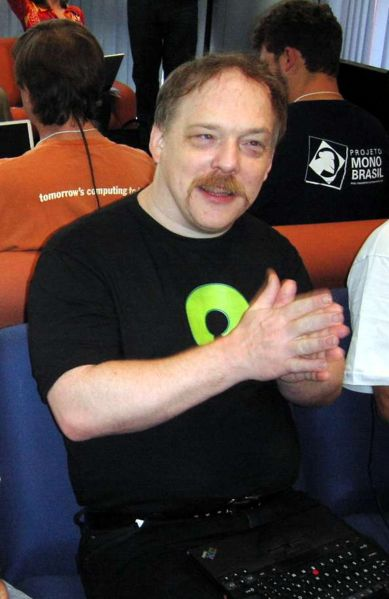
\includegraphics[width=2cm]{figs/EricrRaydmon.jpg}
\end{center}


\begin{itemize}
\item December 4, 1957
\item Fetchmail, gpsd, emacs editing modes
\item "The Cathedral and the Bazaar", published in 1997 -> Became a prominent voice in the open source movement 
\item Co-founded the Open Source Initiative in 1998

\end{itemize}

\end{frame}


\begin{frame}
\frametitle{Origins}

\begin{itemize}
\item First version of the paper written in 1997.
\item Several revisions published until 2000.
\item The author unveils a ``development model'' through the history
  of the Linux kernel and one of his own tools.
\item This model is presented as revolutionary, since it is useful to
  build large systems without apparently any or few organization at all.
\end{itemize}

\end{frame}

\begin{frame}
\frametitle{The models}

\begin{itemize}
\item {\bf The Cathedral}: The ``classic'' model.
\begin{itemize}
\item Closed environment.
\item Small group of leaders/developers.
\item Only ``stable'' releases on, in some cases, ``betas''.
\item Used both in classic development models, such as waterfall, spiral etc;
  and classic FLOSS projects.
\item Examples: GCC, GNU Emacs.
\end{itemize}

\item {\bf The Bazaar}: The model introduced by Linus Torvalds.
\begin{itemize}
\item Open environment, almost any person can participate.
\item There are no clear leaders, undefined number of developers.
\item However, there is a benevolent-dictator figure.
\item ``Release early, Release often''.
\item Examples: Linux.
\end{itemize}
\end{itemize}

\end{frame}

\begin{frame}
\frametitle{The surprise}

The Bazaar style of development:
\begin{itemize}
\item with a community seemed to resemble a large babbling bazaar of
  diverse agendas and approaches
\item with archive repositories where anyone can propose a
  modification
\item but from this, a stable and coherent large system emerges.
\end{itemize}

This was surprising:
\begin{itemize}
\item Why Linux did not fly apart in confusion...?
\item ...and why Linux seemed to go from strength to strength at a speed
  barely imaginable to cathedral-builders?
\end{itemize}

\end{frame}

\section{The Lessons}

\begin{frame}
\frametitle{Lesson 1}

\begin{center}
{\large Every good work of software starts by scratching a developer's
  personal itch.}
\end{center}

\begin{itemize}
\item Most successful free software projects have been started by developers
with needs addressed by their ``pet'' project.
\item In the world of proprietary software, programmers spend their
  time building programs that they neither need nor want.
\item This motivation could explain the high quality of results given
  by Linux.
\end{itemize}

\end{frame}

\begin{frame}
\frametitle{Lesson 2}

\begin{center}
{\large Good programmers know what to write. Great ones know what to
  \textit{rewrite} (and reuse).}
\end{center}

\begin{itemize}
\item Linus Torvalds did not try to write Linux from scratch. Instead,
  he started by reusing Minix code and ideas.
\item Although today all
  reused Minix code has been removed or rewritten, while it was there,
  it provided scaffolding for the infant that would eventually become
  Linux.
\item The source-sharing tradition of the Unix world has always been
  friendly to code reuse.
\end{itemize}

\end{frame}

\begin{frame}
\frametitle{Lesson 3}

\begin{center}
{\large ``Plan to throw one away; you will, anyhow.''}
\end{center}
from chapter 11, The Mythical Man-Month, by Fred Brooks.

\begin{itemize}
\item We really do not understand the problem, until the first
  implementation is done.
\item So if you want to get it right, be ready to start over at least once.
\end{itemize}

\end{frame}

\begin{frame}
\frametitle{Lesson 4}

\begin{center}
{\large If you have the right attitude, interesting problems will find you.}
\end{center}

\begin{itemize}
\item Eric's problem was that he needed a POP protocol client to work
  with.
\item And he found an abandoned one.
\item The problem was the continuation of the abandoned client, and
  Eric took it over and started to coordinate it.
\end{itemize}

\end{frame}

\begin{frame}
\frametitle{Lesson 5}

\begin{center}
{\large When you lose interest in a program, your last duty to it is to hand it off to a competent successor.}
\end{center}

\begin{itemize}
\item Before abandoning the development of a free software,
  we should find another person to continue its development.
\item Fortunately, in the bazaar world, some other hacker will find
  your abandoned work soon, and will start to develop it for his own
  needs.
\end{itemize}

\end{frame}

\begin{frame}
\frametitle{Lesson 6}

\begin{center}
{\large Treating your users as co-developers is your least-hassle route to rapid code improvement and effective debugging.}
\end{center}

\begin{itemize}
\item In Linux, some users are also hackers.
\item Thanks to source code availability, these users can be {\em
    effective} hackers.
\item This can be useful for shortening debugging time.
\item These users will diagnose problems, suggest fixes, and help in
  improvements.
\end{itemize}

\end{frame}

\begin{frame}
\frametitle{Lesson 7}

\begin{center}
{\large Release early. Release often. And listen to your customers.}
\end{center}

\begin{itemize}
\item This is another Linux characteristic: during very active
  development periods, lots of versions were released.
\item Sometimes, more than one in a day.
\item This maintains the hackers constantly stimulated and rewarded:
\item stimulated by the prospect of having an ego-satisfying piece of the action,
\item and rewarded by the sight of constant (even daily) improvement
  of their work.
\end{itemize}

\end{frame}

\begin{frame}
\frametitle{Lesson 8}

\begin{center}
{\large Given a large enough beta-tester and co-developer base, almost
  every problem will be characterized quickly and the fix becomes obvious to
  someone.}
\end{center}

\begin{itemize}
\item ``Given enough eyeballs, all bugs are shallow.'' (named ``Linus's
  Law'' by Eric S. Raymond).
\item Somebody finds the problem, and somebody else understands (and
  fixes) it.
\item The differences between the cathedral and the bazaar: In the
  cathedral-builder view of programming, bugs and development problems
  are tricky, insidious, deep phenomena.
\item In the bazaar, bugs are generally shallow phenomena (they turn
  shallow when exposed to a thousand eager co-developers collaborating
  in next release).
\end{itemize}

\end{frame}

\begin{frame}
\frametitle{Lesson 9}

\begin{center}
{\large Smart data structures and dumb code works a lot better than
  the other way around.}
\end{center}

\begin{itemize}
\item It is difficult to understand the code written by others,
\item but when we understand the data structures, understanding the
  code is easier.
\end{itemize}

\end{frame}

\begin{frame}
\frametitle{Lesson 10: Eric tries the model}

Eric S. Raymond tries successfully the model, with the following
principles:
\begin{itemize}
\item Releasing early and often.
\item Adding everyone who contacted him about the
  implemented program to the beta list.
\item Announcing new releases to the beta list, stimulating people to
  participate.
\item Listening to beta-testers, polling them about design decisions
  and taking in consideration patches and other feedback from them.
\end{itemize}

The consequence:
\begin{center}
{\large If you treat your beta-testers as your most
  valuable resource, they may become that, eventually.
}
\end{center}

\end{frame}

\begin{frame}
\frametitle{Lessons 11 and 12}

\begin{center}
{\large The next best thing to having good ideas is recognizing good
  ideas from your users. Sometimes the latter is better.
}
\end{center}

\begin{center}
{\large Often, the most striking and innovative solutions come from
  realizing that your concept of the problem was wrong.}
\end{center}

\begin{itemize}
\item Eric learned this when saw good ideas for his application
  suggested by users.
\item These ideas helped him to understand that, initially, he was
  looking the solution for the wrong problem.
\end{itemize}

\end{frame}

\begin{frame}
\frametitle{Lesson 13}

\begin{center}
{\large ``Perfection (in design) is achieved not when there is nothing more to add, but rather when there is nothing more to take away.''}
\end{center}
by Antonie de Saint-Exupery.

\begin{itemize}
\item When the code is getting both better and simpler, that is when
  we know it is right.
\item At this moment, the software maintained by Eric was, not only
  very different, but also simpler and better. It was time to change
  its name and give it its new identity: ``fetchmail'' instead of
  ``popclient''.
\end{itemize}

\end{frame}


\begin{frame}
\frametitle{Lessons 14, 15}

\begin{center}
{\large Any tool should be useful in the expected way, but a truly
  great tool lends itself to uses you never expected.}
\end{center}

\begin{center}
{\large When writing gateway software of any kind, take pains to
  disturb the data stream as little as possible -- and never throw away information unless the recipient forces you to!.}
\end{center}

\end{frame}

\begin{frame}
\frametitle{Lessons 16, 17}

\begin{center}
{\large When your language is nowhere near Turing-complete, syntactic
  sugar can be your friend.}
\end{center}

\begin{center}
{\large A security system is only as secure as its secret. Beware of
  pseudo-secrets.}
\end{center}

\begin{itemize}
\item These are lessons learned directly from the concrete
  application: {\em fetchmail}. Not related with SE.
\end{itemize}

\end{frame}

\begin{frame}
\frametitle{Lessons 18, 19}

\begin{center}
{\large To solve an interesting problem, start by finding a problem
  that is interesting to you.}
\end{center}

\begin{center}
{\large Provided the development coordinator has a communications
  medium at least as good as the Internet, and knows how to lead
  without coercion, many heads are inevitably better than one.}
\end{center}

\end{frame}

\section{Criticism}

\begin{frame}
\frametitle{Criticism}

\begin{itemize}
\item No scientific rigor (it is an essay).
\item Based on anecdotal evidences (not a systematic study).
\item Raymond tries to generalize the case of Linux to all free
  software projects.
\item Some critics say that Linux is, in fact, an example of cathedral
  process: there is a leader, and a hierarchic structure of people
  with delegated tasks. Also, responsibilities are distributed in that
  structure although not explicitly.
\end{itemize}

\end{frame}

\begin{frame}
\frametitle{Criticism}

\begin{itemize}
\item Free Software == Bazaar?
\begin{itemize}
\item Is there one development model for free software?
\item Are all projects really built from many contributions of *many*
  developers?
\end{itemize}
\item Bazaar definition may not be accurate.

\item Free Software is not actually a bazaar.

\begin{itemize}
\item Free software is software released with the four freedoms.
\end{itemize}

\end{itemize}

\end{frame}


\begin{frame}
\frametitle{A Second Look at the Cathedral and the Bazaar (Nikolai Bezroukov)}

\begin{itemize}

\item \emph{Brooks Law still apply to Internet-based distributed development}
	\begin{itemize}
	\item Internet only increases the quality of the pool of developers
	\end{itemize}

\item \emph{Given enough eyeballs, all bugs are shallow}
\item \emph{Does Linux belongs to the Cathedral model or to the Bazaar model?}
	\begin{itemize}
		\item A not so democratic Bazaar
		\item Kernel core Cathedral?
	\end{itemize}

\item Does OSS development model automatically yield the best results?

\end{itemize}

\end{frame}



\begin{frame}
\frametitle{Eric Raymond Influence}

\begin{itemize}

\item Netscape Communications
	\begin{itemize}
	\item 22 January, 1998
	\item Netscape publicly released the source code of Netscape Communicator 4.0
	\item \emph{On behalf of everyone at netscape, I want to thank you for helping us get to this point in the first place. Your thinking and writings were fundamental inspirations to our decision.} Eric Hahn, executive vice president and chief technology officer at Netscape
	\end{itemize}
	
\item Wikipedia
	\begin{itemize}
	\item Another great example of large-scale collaboration
	\item \emph{..opened my eyes to the possibility of mass collaboration} - Jimmy Wales, a cofounder of the encyclopedia
	\end{itemize}


\end{itemize}

\end{frame}


\begin{frame}
\frametitle{References}

{\small
\begin{itemize}
\item Eric S. Raymond, ``The Cathedral and the Bazaar'' (1997-2006)
  \url{http://www.catb.org/~esr/writings/cathedral-bazaar/}
\item N. Bezroukov, ``A Second Look to the Cathedral and the Bazaar''
  (1999) \url{http://pascal.case.unibz.it/retrieve/3464/Bazaar.htm}
\end{itemize}
}

\end{frame}

\end{document}

%
% $Id: slides.tex 4228 2006-06-21 21:55:12Z jjamor $
%
%
% Compilar a .pdf con LaTeX (pdflatex)
% Es necesario instalar Beamer (paquete latex-beamer en Debian)
%

%
% Gráficos:
% Los gráficos pueden suministrarse en PNG, JPG, TIF, PDF, MPS
% Los EPS deben convertirse a PDF (usar epstopdf)
%

\documentclass{beamer}
\usetheme{Warsaw}
\usebackgroundtemplate{
\includegraphics[width=\paperwidth]{format/libresoft-bg.png}}
\usepackage[spanish]{babel}
\usepackage[utf8]{inputenc}
\usepackage{graphics}
\usepackage{amssymb} % Simbolos matematicos

%\definecolor{libresoftgreen}{RGB}{162,190,43}
%\definecolor{libresoftblue}{RGB}{0,98,143}

%\setbeamercolor{titlelike}{bg=libresoftgreen}

%% Metadatos del PDF.
\hypersetup{
  pdftitle={Free Software Developers},
  pdfauthor={José Gato, Teo Romera},
  pdfcreator={GSyC/Libresoft},
  pdfproducer=PDFLaTeX,
  pdfsubject={Free Software Engineering},
}
%%

\begin{document}

\title{Free Software Developers}
\subtitle{Master on Free Software}
\institute{\{jgato,teo\}@gsyc.es\\
GSyC/LibreSoft}
\author{José Gato, Teo Romera}
\date{28-29 November 2008}

\frame{
\maketitle
\begin{center}

\includegraphics[width=6cm]{format/gsyc-urjc}
\end{center}
}


% Si el titulo o el autor se quieren acortar para los pies de página
% se pueden redefinir aquí:
%\title{Titulo corto}
%\author{Autores abreviado}


%% LICENCIA DE REDISTRIBUCION DE LAS TRANSPAS
\frame{
~
\vspace{4cm}

\begin{flushright}
{\tiny
(cc) 2008-2010 José Gato, Teo Romera\\
(cc) 2007 Juanjo Amor, Gregorio Robles \\
  Some rights reserved. This work licensed under Creative Commons
  Attribution-ShareAlike License. To view a copy of full license, see
  http://creativecommons.org/licenses/by-sa/2.0/ or write to
  Creative Commons, 559 Nathan Abbott Way, Stanford,
  California 94305, USA.
%  Este documento (o uno muy similar) está disponible en \\
%  \url{http://gsyc.escet.urjc.es/~jjamor/}
}
\end{flushright}
}
%%


\section{Introduction}

\begin{frame}
\frametitle{FLOSS developers are nerds!}

\begin{center}
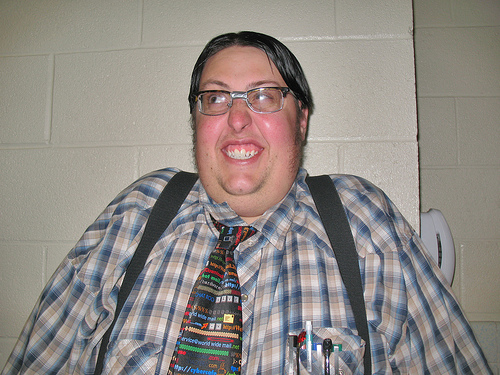
\includegraphics[width=8cm]{figs/nerd.jpg} \\
(Photo: Nerd, by The Infamous Gdub\\
\url{http://flickr.com/photos/theinfamousgdub/1765952198/})
\end{center}

\end{frame}

\begin{frame}
\frametitle{FLOSS developers are gods!}

\begin{center}
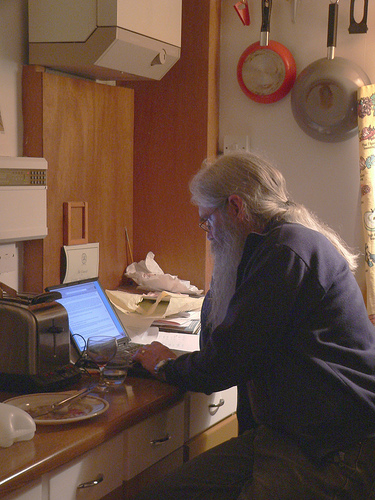
\includegraphics[width=4cm]{figs/hacker.jpg} \\
(Photo: Nerd, or perhaps hacker or geek?, by florriebassingbourn\\
\url{http://flickr.com/photos/75166820@N00/145258818/})
\end{center}

\end{frame}

\begin{frame}
\frametitle{Who are the Free Software Developers?}

\begin{itemize}
\item The open development model allow a large amount of work done by volunteer
developers
\item The possibility of having micro-contributions makes it difficult to know
more about developers
\item The distributed nature of the developer population makes it difficult to
know more about developers
\item Hence, there has been a lack of knowledge about the developers until
recently
\end{itemize}

\end{frame}


\begin{frame}
\frametitle{Who are the Free Software Developers?}

Questions to be answered:

\begin{itemize}
\item Who are the Free Software Developers? (gender, age, cultural level...)
\item Why do they develop Free Software?
\item Do they earn money when developing?
\item Where do they come from?
\end{itemize}

There have been many surveys since 2001 on this issue: WIDI (2001), FLOSS
(2002), FLOSS-US (2003), BCG Hacker Survey (2003), etc.

\end{frame}


\section{Personal Features}

\begin{frame}
\frametitle{Gender}

\begin{itemize}
\item 98\% male
\item 2\% female
\item (The statistical error lies around 3.5\%)
\item Does any discrimination exist? (see Krieger et al.)
\end{itemize}

\end{frame}

\begin{frame}
\frametitle{Age of Free Software Developers}

\begin{center}
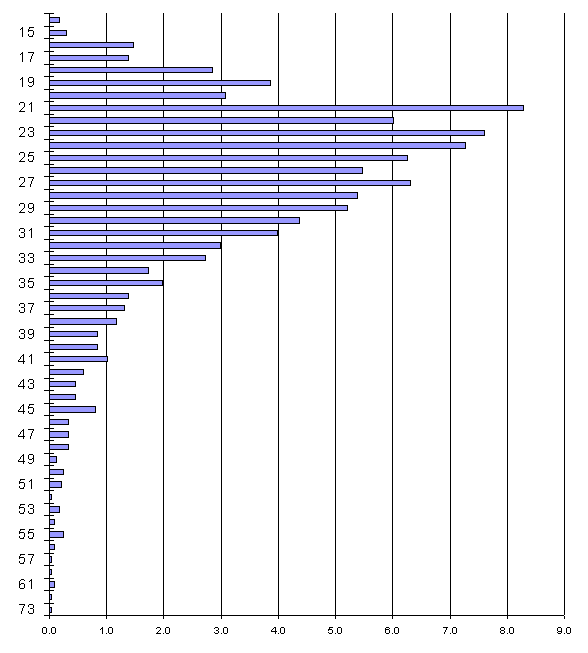
\includegraphics[width=6cm]{figs/age.png}
\end{center}

\end{frame}


\begin{frame}
\frametitle{Starting Age of Free Software Developers}

\begin{center}
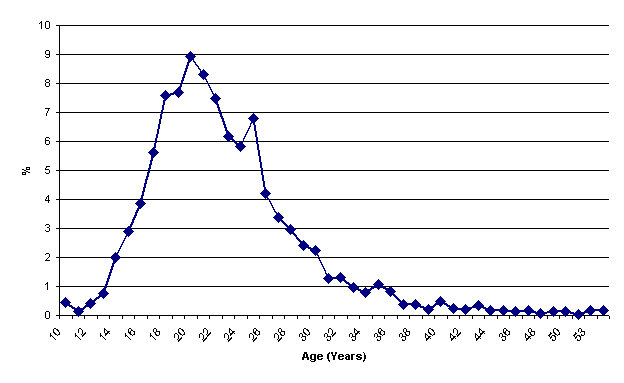
\includegraphics[width=8cm]{figs/starting-age.png}
\end{center}

\end{frame}


\begin{frame}
\frametitle{Educational Background of Free Software Developers}

\begin{center}
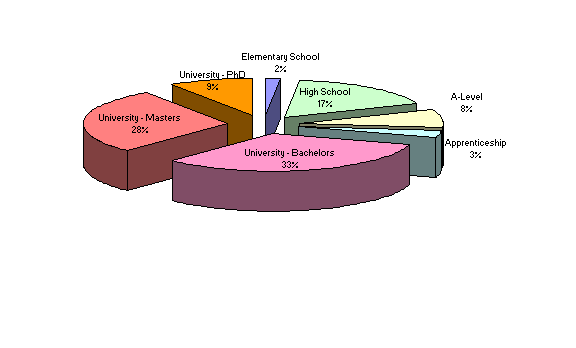
\includegraphics[width=10cm]{figs/educational-background.png}
\end{center}

\end{frame}


\begin{frame}
\frametitle{Professional Background of Free Software Developers}

\begin{center}
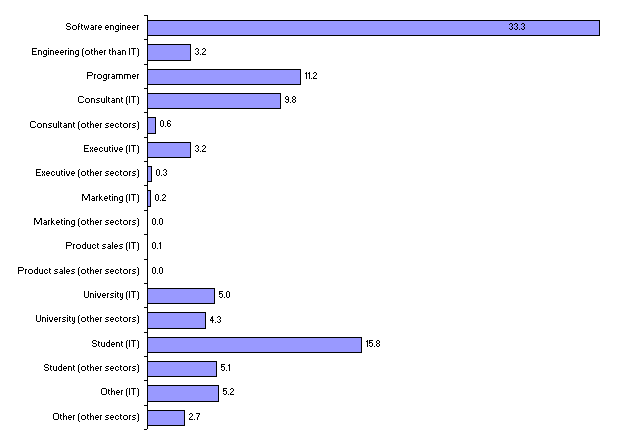
\includegraphics[width=8cm]{figs/professional-background.png}
\end{center}

\end{frame}


\section{Contribution attributes}

\begin{frame}
\frametitle{Time devoted to libre software projects}

\begin{center}
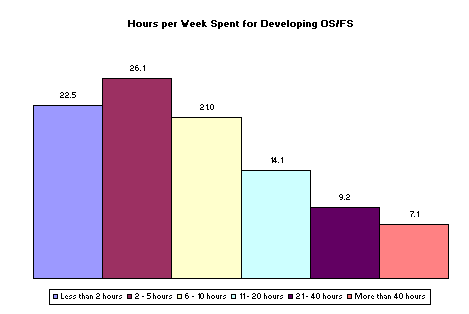
\includegraphics[width=8cm]{figs/hours-week.png}
\end{center}

\end{frame}

\begin{frame}
\frametitle{Time devoted to libre software projects compared to Proprietary Software}

\begin{center}
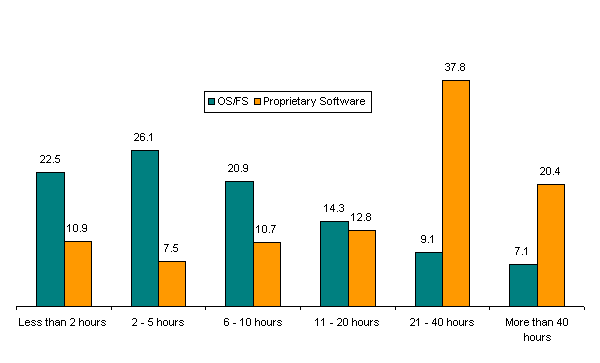
\includegraphics[width=8cm]{figs/TimeOSvsPS.png}
\end{center}

\end{frame}


\begin{frame}
\frametitle{Leadership and reputation}

\begin{center}
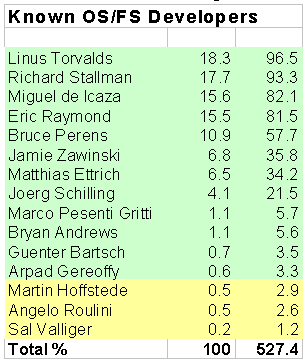
\includegraphics[width=6cm]{figs/leadership.png}
\end{center}

\end{frame}


\begin{frame}
\frametitle{Why Developers Join and Stay developing FLOSS}

\begin{center}
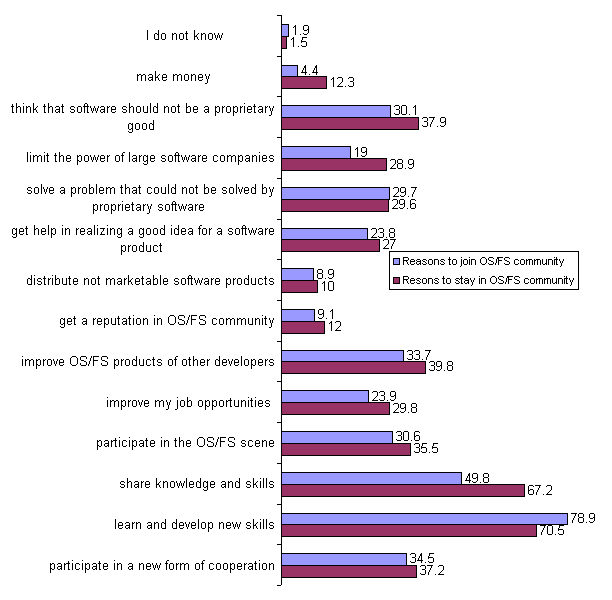
\includegraphics[width=7cm]{figs/why.png}
\end{center}

\end{frame}

\begin{frame}
\frametitle{Monetary rewards from developing FLOSS}

\begin{center}
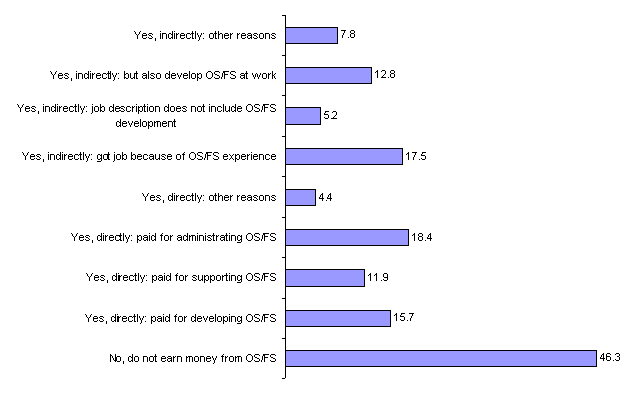
\includegraphics[width=9cm]{figs/money.png}
\end{center}

\end{frame}


\begin{frame}
\frametitle{Alignement Free Software vs. Open Source}

\begin{center}
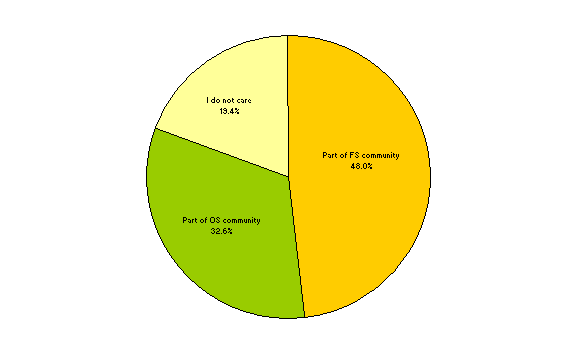
\includegraphics[width=9cm]{figs/FSvsOS.png}
\end{center}

\end{frame}


\begin{frame}
\frametitle{Alignement Free Software vs. Open Source}

\begin{center}
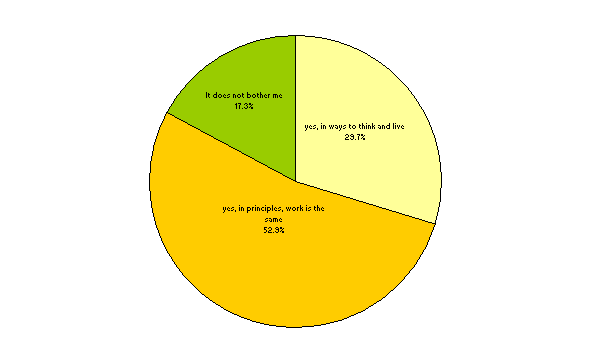
\includegraphics[width=9cm]{figs/FSvsOS2.png}
\end{center}

\end{frame}


\section{Geographic Origin}

\begin{frame}
\frametitle{Geographic Origin of FLOSS developers}

\begin{center}
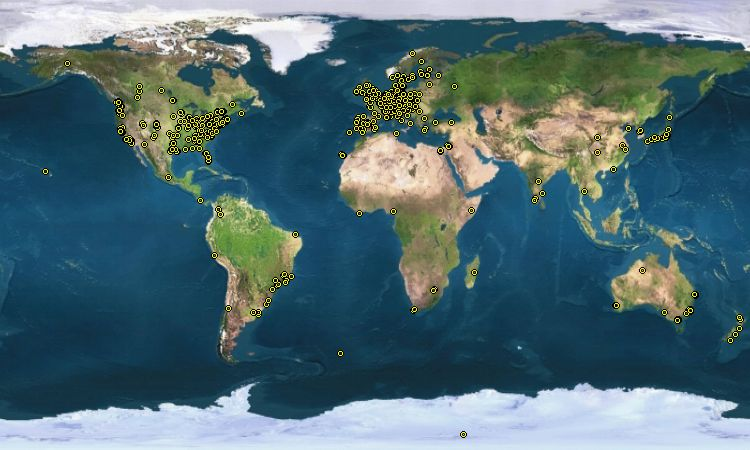
\includegraphics[width=11cm]{figs/developers-map.jpg}
\end{center}

\end{frame}

\begin{frame}
\frametitle{Conclusions}

The average developer

\begin{itemize}
\item Young male with a university degree
\item Tight link of the university with FLOSS
\item Pareto's Law in dedication hours
\item Non-monetary, non-egocentric motivations
\item Main motivation: sharing and learning
\item Good coding does not always mean reputation
\end{itemize}
\end{frame}

\begin{frame}
\frametitle{They are just normal people}

\begin{center}
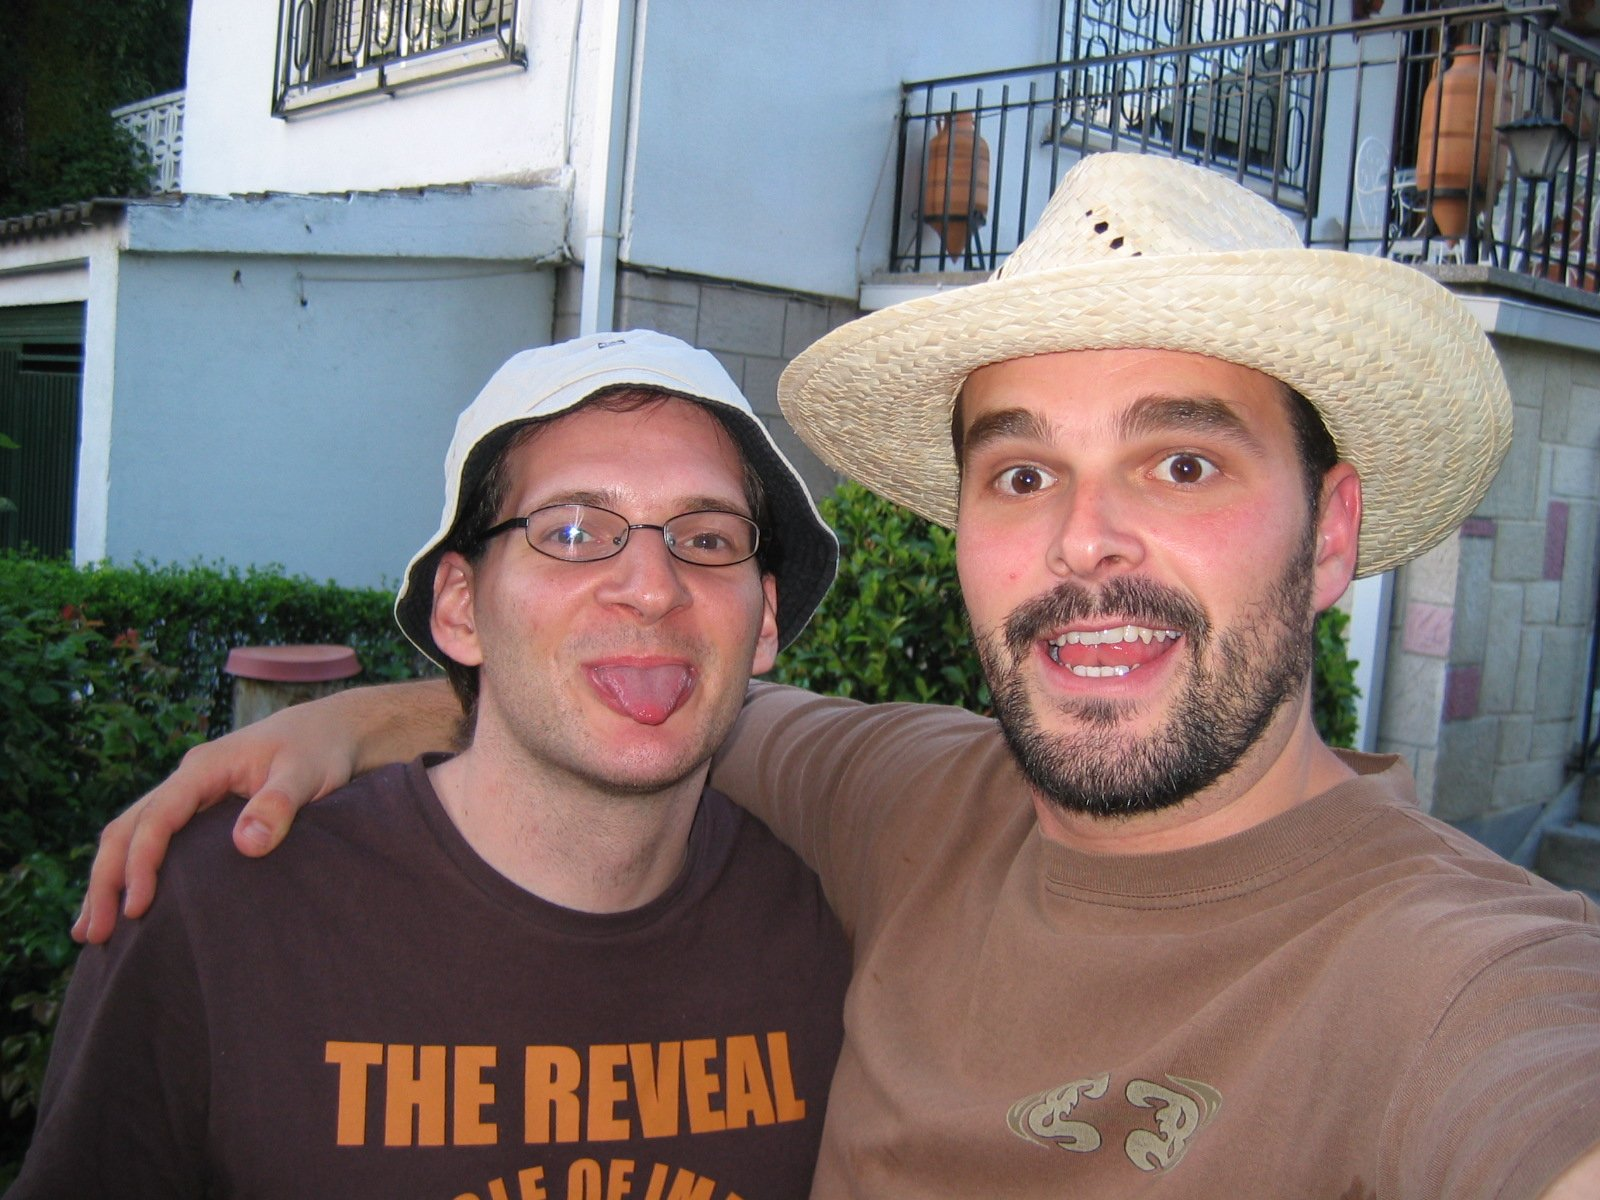
\includegraphics[width=8cm]{figs/martin.jpg}
\end{center}

\end{frame}

\end{document}



\end{document}
